% EAJ - svg generation needs to be run with -shell-escape:
% pdflatex -shell-escape filename.tex
\documentclass[border=2pt, tikz, convert={command=\unexpanded{{pdf2svg \infile\space "\jobname.svg" && rsvg-convert --zoom 1.85 --format svg --output "\jobname.svg" "\jobname.svg" && convert -density 300 \infile\space "\jobname.png"}}}]{standalone}
\begin{document}
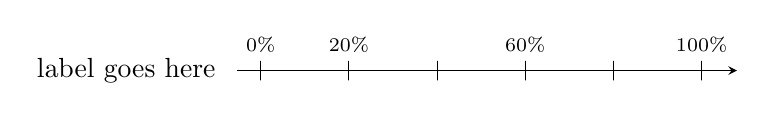
\begin{tikzpicture}

%  TikZ Styles for Number Lines
\tikzset{
  tickLabelAbove/.style={
      font=\small,        % Font size for tick labels
      anchor=mid,         % Baseline align text vertically across nodes
      yshift=2.0ex,       % Vertical offset for labels above the line
  },
  tickLabelBelow/.style={
      font=\small,        % Font size for tick labels
      anchor=mid,         % Baseline align text vertically across nodes
      yshift=-2.6ex,      % Slightly larger offset below the line to account 
                          % for the label's baseline alignment (ensures visual balance).
  },
  numLineTick/.style={
      draw,               % Draw tickmark node
      minimum width=0pt,  % No width for the node box
      minimum height=7pt, % Height of the tickmark
      line cap=round,     % Rounded ends for ticks
      inner sep=0pt,      % No inner padding
      outer sep=2pt,      % Space around the tick
      line width=0.35pt,  % Thickness of the tick line
  },
}

% Parameters
\def\lineWide{2.5in} % width of line (not including label)
\def\numLineExtra{0.3cm} % Hardcoded extra space at the ends
\def\numMarks{6}

\coordinate (leftEnd) at (0, 0);
\coordinate (rightEnd) at (\lineWide, 0);
\draw[->, >=stealth] (leftEnd) -- (rightEnd);
\node[anchor=east, xshift=-0.15cm] at (leftEnd) {label goes here};

% draw ticks as nodes (mark-n). 1st mark is (mark-1).
\foreach \x in {1,...,\numMarks}{%
    \node[numLineTick] (mark-\x) at ({\numLineExtra+(\x-1)*(\lineWide-2.5*\numLineExtra)/(\numMarks-1)},0) {};
}

\def\labels{0\%,20\%, , 60\% , ,100\%}
\foreach \label [count=\i] in \labels {
    \node[above=3pt,font=\scriptsize] at (mark-\i) {\label};
}


\end{tikzpicture}
\end{document}